\section{Introduction}
Materialized views, stored pre-computed query results, are a well-known approach to speed- and scale-up query processing \cite{LarsonY85, gupta1995maintenance, chirkova2011materialized, halevy2001answering}.
During the last 30 years, the research community has thoroughly studied the approach, and all major database vendors have added support for them. 
As data grows, materialized views have become increasingly useful and have been the subject of numerous recent works \cite{lefevre2014opportunistic, bailis2014scalable, perez2014history}.
More recent work expands the developed techniques to data analytics problems and, for example, shows remarkable results for linear algebra and machine learning \cite{nikolic2014linview, zhang2014mat}.

However,when base tables are updated, materialized views face the problem of \emph{staleness}. 
A well-studied efficient solution is incremental view maintenance \cite{gupta1995maintenance, chirkova2011materialized}.
Instead of re-calculating the whole view for every update, incremental view maintenance reduces the cost by calculating only the incremental changes from one view to the next updated view. 
In the Big Data era, new data arrives at an increasingly fast rate, and for frequently changing tables, even incremental maintenance can be expensive; every update to one of the {\em base} tables requires updating all the dependent views. 
%Still, for many applications, even incremental maintenance can be too expensive. 
%This is particularly true for very fast changing tables and/or complex views. 
Furthermore, recent database systems are often distributed across machines, further amplifying the challenge. 
Consequently, it is common to defer the maintenance to a later time \cite{chirkova2011materialized, zhou2007lazy}.
Deferral allows for many advantages such as batching updates together to amortize overheads and scheduling updates at times when there are more system resources available, for example, at night.
While deferral has compelling benefits, it does not guarantee up-to-date results between maintenance periods. 

\begin{figure}[t] %\vspace{-1.5em}
\centering
 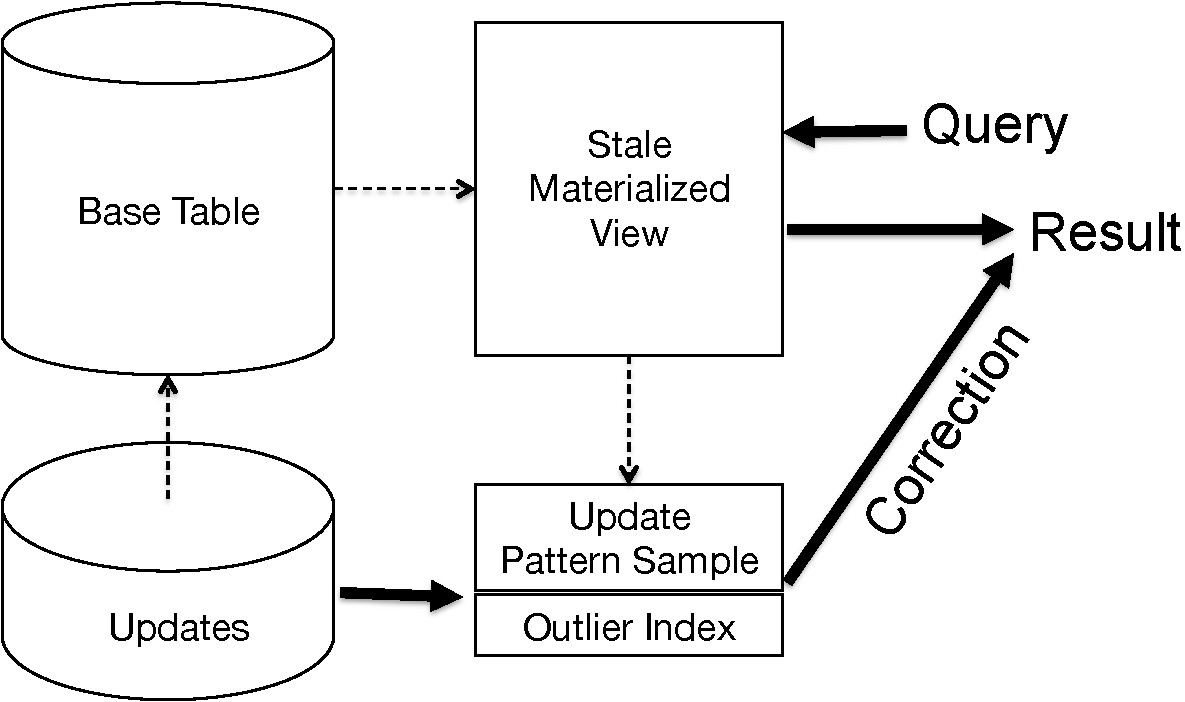
\includegraphics[scale=0.30]{figs/sys-arch.pdf}
 \caption{SVC has three main components: (1) sampling, (2) correction, and (3) outlier indexing. From a sample of up-to-date data, we estimate
 a correction for queries on stale materialized views. To make this process robust to outliers, we apply a technique called outlier indexing. \label{sys-arch}}\vspace{-1.5em}
\end{figure}

As a materialized view becomes more stale, queries on the view become increasingly inaccurate.
This closely mirrors the problem of dirty data where data errors can reduce the accuracy of query results, and data cleaning has been proposed to mitigate such inaccuracy \cite{rahm2000data}.
%Numerous data cleaning approaches have been proposed to to efficiently clean data errors and improve the accuracy of query results.
In this work, we explore whether refreshing stale rows in a materialized view can be modeled as a data-cleaning problem.
We take inspiration from recent results from the SampleClean data-cleaning framework which show that instead of cleaning the entire dataset,
it suffices to clean a small sample of dirty records to greatly improve query accuracy \cite{wang1999sample}.
This data-cleaning perspective raises a new possibility for materialized views, namely, that we can return more accurate results without incurring the cost of full view maintenance.
However, staleness is different sort of data error that raises interesting new challenges in sampling, cleaning, and efficient query processing.

%Recent results in data cleaning increasingly consider the costs of data cleaning .

%The results show that 

%Materialized views, stored pre-computed query results, are used to facilitate fast query processing on large datasets \cite{gupta1995maintenance, chirkova2011materialized, halevy2001answering}.
%Materialization and related concepts such as selecting queries to materialize
%have been well studied in recent research \cite{zaharia2012resilient,lefevre2014opportunistic, bailis2014scalable, perez2014history}.
%This research has further expanded beyond the SQL setting \cite{nikolic2014linview, zhang2014mat} and 
%has shown promising results when applied to numerical linear algebra and machine learning.
%However, when derived from frequently changing tables,
%materialized views face the challenge of \emph{staleness} where the pre-computed results need to be updated.
%To avoid expensive recalculation, incrementally updating the views,
%also called incremental maintenance, has been well studied \cite{gupta1995maintenance, chirkova2011materialized}.

%Unfortunately, in many applications, incremental maintenance on each update can be very costly. 
%Consequently, it is common to defer maintenance to a later time \cite{chirkova2011materialized, zhou2007lazy}.
%Deferral allows for many advantages such as batching updates together to amortize overheads and scheduling updates at times when there are more system resources available, for example, at night.
%Deferral allows for increased flexibility to meet the resource constraints of the system, but may not guarantee that the view will be up-to-date.

%When a materialized view is out-of-date during a maintenance gap, queries issued to the view can have \emph{stale} results. 

%In this work, we address the view-maintenance problem from a different perspective.
%We explore whether refreshing stale rows in a materialized view can be modeled as a data-cleaning problem and whether stale query results can be \emph{cleaned}.
%While much of the data cleaning literature focuses on improving query accuracy on dirty datasets,
%recent work has also considered the costs of data cleaning \cite{wang1999sample}.


We propose Sample-View-Clean (SVC), a framework that uses a \emph{sample} of up-to-date data to \emph{correct} stale aggregation query results.
While approximate, the corrected query result can be bounded within confidence intervals.
This framework will be complementary to existing deferred maintenance approaches; when the materialized views are stale between maintenance cycles, we can apply SVC for approximate results for a far smaller cost than having to maintain the entire view.
SVC gives results that are fresh and the user controls a bounded approximation error with the sampling ratio.

%Sampling gives the user the ability to scale the performance 
%Existing techniques allow the user to control the freshness of queries by chaning maintenance parameters (e.g. nightly maintenance vs. hourly maintenance) based on prior experience. However, without bounds on the results, a burst of updates can lead to unexpected changes in query accuracy.
%On the other hand, our approach gives results that are, in expectation, fresh and the user controls the tightness of the bound with the sampling ratio.

%The SampleClean project [?] studied a related problem of bounding aggregate queries on dirty datasets but did not consider materialized views or the effect of missing records.

In Figure \ref{sys-arch}, we highlight the three main components of SVC: (1) sampling, (2) correction, and (3) outlier indexing. In (1), we define an ``update pattern" which represents how an update affects the view, and we sample these patterns. (2)  From the sample, we estimate how much the updates affect the query and we use this estimate to clean the stale query result.
Finally, in (3) sampling is known to be sensitive to outliers \cite{chaudhuri2001overcoming}.
We utilize a technique called outlier indexing \cite{chaudhuri2001overcoming}, which guarantees that rows in the materialized view derived from an ``outlier" record (one that has abnormal attribute values) is contained in the sample, which can be used to increase correction accuracy.

%Our approach can be implemented with a relatively small overhead: at maintenance time the generation of random numbers to build the sample, and at query execution time single pass over a small sample of data to estimate a correction for the query.
%Consequently, sampling can significantly save on maintenance costs and give a flexible tradeoff between accuracy and performance.
To summarize, our contributions are as follows:

\begin{itemize}\vspace{-.45em}
\item We model the incremental maintenance problem as a data cleaning problem and staleness as a type of data error.\vspace{-.45em}
\item We define the concept of ``update patterns", a logical unit that represents how an update affects a materialized view, and show how to sample the update patterns. \vspace{-.45em}
\item Using a sample of update patterns, we can correct stale aggregation queries on materialized views with bounded accuracy.\vspace{-.45em}
\item We use an outlier index to increase the accuracy of the approach for power-law, long-tailed, and skewed distributions.\vspace{-.45em}
\item We evaluate our approach on real and synthetic datasets in both single-node and distributed environments.\vspace{-.45em}
\end{itemize}

The paper is organized in the following way. 
In Section~\ref{sec-background}, we introduce materialized views and discuss the current maintenance challenges.
Next, in Section~\ref{sec-arch}, we give a brief overview of our overall system architecture.
In Section~\ref{sampling} and~\ref{correction}, we describe the sampling and query processing of our technique.
In Section~\ref{outlier}, we describe the outlier indexing framework.
In Section~\ref{sec:ext}, we discuss how our framework extends to Select queries and deletions.
Then, in Section~\ref{exp}, we evaluate our approach.
Finally, we end with our Related Work in Section~\ref{related} and our Conclusions and Future Work in Section~\ref{conclusion}.

\iffalse
 These two pieces can be costly in different
applications. (1) In distributed environments where the view is partitioned
over a cluster, incremental view maintenance often necessitates communicating
the delta view. (2) Systems such as Apache Spark, Cloudera Impala,
and Apache Tez {[}?{]} offer materialized view support, however, are
not optimized for selective updates nor have native support for indices.
This can lead to high maintenance costs in applications where the
views are derived from joins that are not aligned with the partitioning
of the base tables. (3) Base data is often raw requiring pre-processing
such as string processing, deserialization, and formatting; all of
which can can be expensive to run on a large number of updates. 



Querying a stale view is similar to problems studied in data cleaning{[}?{]}.
When databases are dirty, query results can be arbitrarily wrong.
Data cleaning is used to remove data errors but this can be very costly either 
requiring machine learning to classify errors or even human intervention.
SampleClean is a query processing framework that answers aggregate
queries on dirty datasets by applying potentially expensive cleaning
techniques to just a sample. The results, while approximate, are bounded
with respect to the clean data and the system offers a flexible tradeoff
between cleaning cost and result accuracy. Similarly, a stale row
and an expensive incremental maintenance scheme, mirrors the problem
setting studied in SampleClean. 

In this paper, we propose a data cleaning approach for approximate,
bounded aggregation queries on stale views. Instead of maintaining
the entire view, we maintain only a small sample of the view. Then
given an aggregation query on this view, from this small sample, we
can estimate how the updates affect the query result. We apply this
estimate to correct the dirty aggregation query result on the stale
data. We call this approach \emph{approximate query correction}. 
These corrections are provably bounded, in contrast to the unbounded staleness,
and the sampling gives a flexible tradeoff to meet performance constraints such as throughput.
Sampling helps reduces both bottlenecks in view maintenance, delta
view calculation and view updating, as it reduces the number of updates
that need to processed and then written.

Another relevant concept from data cleaning is outlier detection {[}?{]}.

In this work, we propose an outlier indexing framework that guarantees that
rows in the materialized view derived from an ``outlier" record, one with
an abnormal attribute value, are included in the sample.

In summary, our contributions are as follows:
\begin{itemize}
\item We present a query processing framework that corrects aggregation queries on stale
views using a sample of up-to-date data.
\item We couple this approach with an oultier indexing framework that allows
for selection queries on outliers and we show both analytically and empirically that 
this can improve query accuracy.
\item We evaluate our approach on two systems, Apache SparkSQL and MySQL,
and discuss how the different systems affect performance performance
parameters.
\end{itemize}
\fi
